
\section{绪论}


正文是学位论文的主体,第一章为绪论,最后一章为结论与展望。我们来测试一个上标引用。
\begin{figure}[H]
\centering
\subfigure[原始图像]{\label{figure:001} 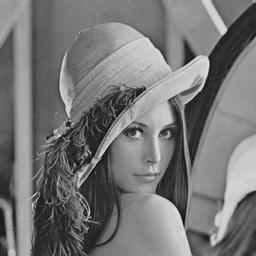
\includegraphics[width=0.4\textwidth]{001}}
\subfigure[噪声图像($\mu=0,\sigma=20$)]{\label{figure:002} 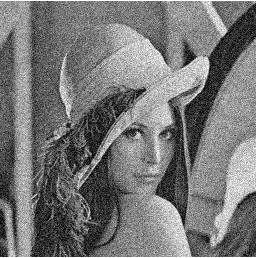
\includegraphics[width=0.4\textwidth]{002}}
\caption{初始图像}
\end{figure}

 \begin{figure}[h]
 \centering
 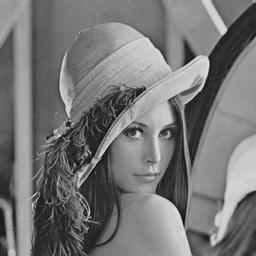
\includegraphics[width=0.5\textwidth,angle=0]{001}
 \caption{这是标题}
 \end{figure}    

    每章标题按一级标题编排,每节标题按二级标题编排,每小节标题按三级标题编排。

    “章”、“节”、“小节”的编号统一为:1、1.1、1.1.1。

    四级以后的标题和编号的编排原则为:下级标题的显目程度不超过上一级,不重复或混淆。

    编号与题目之间空一格。

    \subsection{二级标题}
    

        积土成山,风雨兴焉;积水成渊,蛟龙生焉;积善成德,而神明自得,圣心备焉。故不积跬步,无以至千里;不积小流,无以成江海。骐骥一跃,不能十步;驽马十驾,功在不舍。锲而舍之,朽木不折;锲而不舍,金石可镂。蚓无爪牙之利,筋骨之强,上食埃土,下饮黄泉,用心一也。蟹六跪而二螯,非蛇鳝之穴无可寄托者,用心躁也。
         

        \subsection{三级标题}

        平林漠漠烟如织,寒山一带伤心碧。暝色入高楼,有人楼上愁。王阶空伫立,宿鸟归飞急。何处是归程,长亭更短亭。


            \subsubsection{四级标题}
                
            君不见,黄河之水天上来,奔流到海不复回。君不见,高堂明镜悲白发,朝如青丝暮成雪。人生得意须尽欢,莫使金樽空对月。天生我材必有用,千金散尽还复来。烹羊宰牛且为乐,会须一饮三百杯。岑夫子,丹丘生,将进酒,君莫停。与君歌一曲,请君为我侧耳听。钟鼓馔玉不足贵,但愿长醉不复醒。古来圣贤皆寂寞,惟有饮者留其名。陈王昔时宴平乐,斗酒十千恣欢谑。主人何为言少钱,径须沽取对君酌。五花马,千金裘,呼儿将出换美酒,与尔同销万古愁。

            \subsubsection{四级标题}

                一屠晚归,担中肉尽,止有剩骨。途中两狼,缀行甚远。

                屠惧,投以骨。一狼得骨止,一狼仍从。复投之,后狼止而前狼又至。骨已尽矣,而两狼之并驱如故。

                屠大窘,恐前后受其敌。顾野有麦场,场主积薪其中,苫蔽成丘。屠乃奔倚其下,弛担持刀。狼不敢前,眈眈相向。

                少时,一狼径去,其一犬坐于前。久之,目似瞑,意暇甚。屠暴起,以刀劈狼首,又数刀毙之。方欲行,转视积薪后,一狼洞其中,意将隧入以攻其后也。身已半入,止露尻尾。屠自后断其股,亦毙之。乃悟前狼假寐,盖以诱敌。

                狼亦黠矣,而顷刻两毙,禽兽之变诈几何哉?止增笑耳。

            \subsubsection{又是一个四级标题}

                孔子东游,见两小儿辩斗。问其故。

                一儿曰:“我以日始出时去人近,而日中时远也。”

                一儿以日初出远,而日中时近也。

                一儿曰:“日初出大如车盖,及日中则如盘盂,此不为远者小而近者大乎?”

                一儿曰:“日初出沧沧凉凉,及其日中如探汤,此不为近者热而远者凉乎?”

                孔子不能决也。

                两小儿笑曰:“孰为汝多知乎?”

